\chapter{How grammatical can you get?}

\section{Noam Chomsky's view(s) about grammaticality}
Another view is evident in Chomsky's very early work. Under this view, there are generative rules. A generative rule is a rule that specifies how to generate a grammatical sentence. If something can be generated by those rules, then it's grammatical, and if it can't it's not. This raises the problems of how we decide what the rules are or should be. In order to figure them out, we need data on what is grammatical and what isn't. Sampson would say, just go and look at a corpus. That's what the LLM-builders have done, and the LLMs seem to have figure this out just fine.

To illustrate the contrast between these two views, it's helpful to first have a better idea of what a generative grammar is. Let's consider a toy version. A generative grammar consists of two parts: a set of rules and a lexicon (a library of words). Here's how a small part of a generative grammar might work:

\subsection{Toy grammar}

\subsubsection*{Lexicon}
\begin{itemize}
 \item Nouns: \{\textit{dog}, \textit{cat}\}
 \item Verbs: \{\textit{chases}, \textit{sees}\}
 \item Determinatives: \{\textit{the}, \textit{a}\}
\end{itemize}

\subsubsection*{Rules}
Generative rules specify what sequences of vocabulary items are grammatical:

\begin{enumerate}
 \item N \(\rightarrow\) \{\textit{dog}, \textit{cat}\}
 \item D \(\rightarrow\) \{\textit{the}, \textit{a}\}
 \item NP \(\rightarrow\) D N
 \item V \(\rightarrow\) \{\textit{chases}, \textit{sees}\}
 \item VP \(\rightarrow\) V NP
 \item S \(\rightarrow\) NP VP
\end{enumerate}

Using the above rules, we can generate a sentence like \textit{The dog chases the cat}. Here's how:

We start with rule 6. This splits S into NP and VP. To produce NP, we use rule 3, and this splits NP into D and N, for which we use rules 2 and 1, respectively. We choose \textit{the} for D and \textit{dog} for N.

Next, we move to VP. VP is produced by invoking rules 5, 4, 3, 2, and 1 in that order. We choose \textit{chases} for V, \textit{the} for the second D, and \textit{cat} for the second N.

Putting this all together, we have generated the sentence \textit{The dog chases the cat} using our toy grammar. Figure \ref{fig:dog-cat} illustrates the structure of this sentence.

%\begin{figure}
% \centering
% 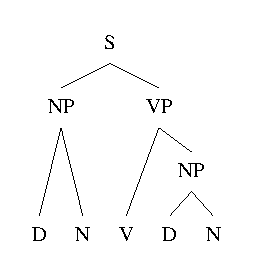
\includegraphics{figures/texstudio_wZsNnD.pdf}
% \caption{A grammatical sentence.}
% \label{fig:S-NP+VP}
%\end{figure}

%To flesh this out using the lexicon, we use the rules to makes choices. For example, to pick \textit{the} for D and \textit{dog} for N. Altogether, this produces the tree in Figure \ref{fig:dog-cat}.

\begin{figure}
 \centering
 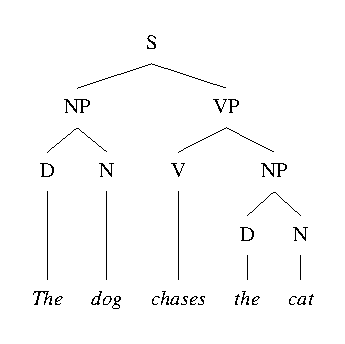
\includegraphics{figures/texstudio_wZsNnD2.pdf}
 \caption{The grammatical sentence \textit{The dog chases the cat}.}
 \label{fig:dog-cat}
\end{figure}

This toy grammar underscores the generative approach to grammaticality. The ability to produce a sentence according to specific rules determines its grammaticality. It contrasts with Sampson's view by implying that not all sentences found in a corpus necessarily reflect underlying grammatical rules. For instance, \textit{The dog the cat sees} cannot be generated and so it is ungrammatical, regardless of whether it appears in corpus data.

Under this generative view, a given sentence is either generated by the grammar and so is grammatical or it isn't and so it's not. It's a binary view of grammaticality.

\section{Grammaticality in Computer Languages}

In high school, my friend Jamie Ramsden and I spent most of our computer science class time programming simple computer games. This was regularly interrupted by our classmates asking us questions about and help with the assignments, which we would do our best to provide.

On one occasion, we realized that we'd left it too late and the assignment was almost due. We very quickly threw together the program, printed out the Basic code, drew the required flowchart -- after the program was written, of course -- and submitted it.

The catch was that we handed in identical code for what was supposed to be an individual assignment. When our teacher, Mr. Boyko, %verify
was handing back the assignments, he asked us if he should give us each 50\% for the perfectly but not independently executed assignment. We agreed that this was a fair way to proceed and then cheekily added that the same allotments should be extended to our proportion of other students' grades, since we'd helped them. In the end, I think we each got full marks.

Mr. Boyko had been able to identify our collaboration because, despite the assignment being quite simple -- perhaps it involved writing a bubble sorting algorithm, which compares and swaps adjacent elements if they are in the wrong order, proceeding through the list multiple times until it is all sorted -- there are many different but functionally equivalent ways it can be written. It would be extremely unlikely that two students would independently produce exactly the same code.

In this way, computer code is similar to human languages. We can tell a story or a bubble sort in many different ways. There are significant differences between the two types of languages though. The output of a bubble sort is either correctly sorted or it's not. There's really no other possible outcome. The telling of a story, on the other hand, can result in a myriad of outcomes.

Recently, some friends and I read \textit{Children of Time}, a 2015 science fiction novel by Adrian Tchaikovsky. Though the three of us read exactly the same book, we had very different understandings of the ending. (spoilers ahead) 

I thought the spiders had simply shared information to manipulate the game-theoretic equilibrium, while my friends understood them to have fundamentally altered the DNA of the humans, such that they were no longer human.

The point is, perhaps, an obvious one: Human languages are often open to many different interpretations and functional equivalence is commonly difficult. Computer code, in contrast, is typically much more deterministic. That's because computers don't share the common ground we do. Even in writing, I can assume that you, dear reader, experience gravity, breathe air, and know that bananas are yellow, and that you have human ancestors, morals, goals, and fears. When it comes to computer languages such as Basic, the only common ground is the very specific meanings of commands and their arguments. 

As a result, not only will every correctly coded bubble sort have the same output but also running any bubble sort, however coded, will have one of only four possible outcomes:

\begin{enumerate}
    \item the output is always correct
    \item the output is correct for some sets and incorrect for others
    \item the output is always incorrect
    \item the program produces no output
\end{enumerate}

In terms of grammaticality, the program either is or it isn't. Though only the first is what was intended, all but the last are the outcomes of ``grammatical'' code.

I'm writing this book in \LaTeX, a software system for typesetting documents. \LaTeX differs from Basic in a number of ways. The first is that the output is highly flexible. If you add one word somewhere, this may result in many subtle adjustments through many lines of text output without the need to change the code. Nevertheless, the output remains deterministic. The second difference is that \LaTeX often handles errors very gracefully rather than stopping when it encounters an error. Instead, it will leave a note in the lot saying that it thinks you forgot to add something and that it added it for you, or saying that something wasn't working and so it was simply ignored. And yet, even when it is able to compensate for my syntax errors, they're still wrong.

Computer languages are meticulously crafted to ensure that each statement or expression carries a singular, unambiguous meaning. This design principle starkly contrasts with the fluidity and multiplicity of meanings found in human languages, where the same phrase can evoke laughter, confusion, or a myriad of other reactions based on context, tone, and the relationship between interlocutors.

When my children were young, they make requests like, ``can you make me a snack?'' A response like, ``Poof, you're a snack," followed by an attempt to eat them would result in many giggles. (That it would not work today is not a fault of the language.) The pun relies on the structural ambiguity between the double-object construction illustrated in \textit{give them \uline{a snack}} and the resultative construction illustrated by \textit{make them \uline{happy}}. In each case, the second complement in the VP -- the underlined one -- may be an NP, but as suggested by the term \textsc{double-object construction}, the underlined NP in that construction has the function of an object, while in the resultative construction, it functions as a predicative complement. Just as a nurse need not be a woman, a predicative complement doesn't have to be an NP; it can also be a bare-role NP, such as \textit{president}, \textit{secretary}, or \textit{treasurer}, or an adjective phrase like \textit{very happy}, \textit{aware}, or \textit{good}.

Punning is just one of the many elements of human language that are entirely absent in the rigid syntax and semantics of computer code. There, a command like \texttt{print("You're a snack")} can only mean one thing. It instructs the computer to display a specific string of characters, nothing more, nothing less. It's not possible for a given string to be ambiguous between two functions such as object and predicative complement.

This also means that, for programming languages, the idea of a construction, a form--meaning linkage, provides little conceptual value. Programmers can't break the rules without breaking the program. They can't creatively use commands in structures with new social or semantic results. And while we can say that a response such as \textit{I have fifty five years} to the question \textit{how old are you?} is formally possible but still ungrammatical, the Basic interpreter cannot make distinctions of that sort. If the Basic program runs, it's grammatical, regardless of the outcome.

Grammaticality in languages like English, Japanese, Hausa, and American Sign Language, though, isn't so black and white.

\begin{enumerate}
    \item A construction may be grammatical in one context and ungrammatical in another.
    \item A construction may be grammatical with a particular meaning and ungrammatical with another.
    \item It may 
\end{enumerate}

When children play, a significant portion of the time is taken up establishing the ground rules -- what is and is not allowed -- and so it was when my kids had friends over. And one thing that struck me about the rule setting I overheard was constructions like *\textit{you're not allowed double-bouncing somebody on the trampoline.} For me, \textit{allow} licenses a \textit{to}-infinitival complement, and the present participials like \textit{bouncing} that the kids in the neighbourhood used were ungrammatical (for them, both were fine).

But I reflected that things could get much worse and came up with (\ref{ex:allowed-dessert}).

\ea \label{ex:allowed-dessert}
    \ea[]{\textit{You're allowed \uline{to have dessert}.}}
    \ex[]{\textit{You're allowed \uline{having dessert}.}}
    \ex[]{\textit{You're allowed \uline{that you have dessert}.}}
    \ex[]{\textit{You're allowed \uline{you have dessert}.}}
    \ex[]{\textit{You're allowed \uline{have dessert}.}}
    \z
\z

Again, for me -- perhaps you feel the same -- (\ref{ex:allowed-dessert}b) is just a little off, (c) gets my full attention, (d) is really shaking things up, and (e) completely throws English grammar out the window. Yet each of the underlined sections is a possible complement in constructions like those in (\ref{ex:allowed-variants}).

\ea \label{ex:allowed-variants}
    \ea[]{\textit{You want \uline{to have dessert}.}}
    \ex[]{\textit{You like \uline{having dessert}.}}
    \ex[]{\textit{We told them \uline{that you have dessert}.}}
    \ex[]{\textit{We let \uline{you have dessert}.}}
    \ex[]{\textit{You can \uline{have dessert}.}}
    \z
\z

How could it be that (\ref{ex:allowed-dessert}) exhibits increasing amounts of ungrammaticality, and why would that happen?


 

\section{}
Most of us, however, do not experience language with such a rigid distinction. Consider the following sentences:

\ea \label{ex:dog-gradience}
 \ea[\phantom{****}]{\textit{The big black dog fetched sticks at the park.}}
 \ex[\phantom{***}\textsuperscript{?}]{\textit{The black big dog fetched sticks at the park.}}
 \ex[\phantom{***}\textsuperscript{?}]{\textit{The black big dog fetched stick at the park.}}
 \ex[\phantom{***}*]{\textit{The black big dog not fetch stick at the park.}}
 \ex[\phantom{**}**]{\textit{Black big dog no fetch stick at park.}}
 \ex[\phantom{*}***]{\textit{Black big dog no fetch park.}}
 \ex[****]{\textit{Dog big no stick no no park fetch.}}
 \z
\z

For me, these sentences do not all seem equally grammatical (as Sampson would suggest) nor does there seem to be a clear binary distinction between the grammatical and ungrammatical. If forced to choose, I think I'd draw a line between (c) and (d), but (d) seems much more grammatical than (g). In other words, the grammaticality of these sentences feels more like a gradient, a spectrum, or a continuum than a binary choice.

But this is perhaps simply because the sentences different numbers of grammatical issues. In (c), the normal order of adjectives \textit{big black} is reversed. In (d), on top of this adjective issue, \textit{sticks} has becomes \textit{stick}. This unusual construction could be analogized to \textit{catch ball}, \textit{jump rope}, or \textit{play guitar}, but it's not conventional the way they are. To this, (e) adds \textit{not} without the auxiliary verb \textit{did} that typically accompanies it, loosing the past-tense marking in the bargain.

What would happen if each sentence had but a single error, as in (\ref{ex:dog-gradience2}?

\ea \label{ex:dog-gradience2}
 \ea[\textsuperscript{?}]{\textit{The \uline{black big} dog fetched sticks at the park.}}
 \ex[*]{\textit{The big black dog \uline{didn't fetched} sticks at the park.}}
 \ex[*]{\textit{\uline{Big black dog} fetched sticks at the park.}}
 \ex[*]{\textit{The big black dog \uline{no fetched} sticks at the park.}}
 \ex[*]{\textit{The \uline{dog big black} fetched sticks at the park.}}
 \ex[*]{\textit{The big black dog fetched sticks at \uline{park the}.}}
 \ex[*]{\textit{The big black dog \uline{fetched sticks the park}.}}
 \ex[*]{\textit{The big black dog \uline{put sticks} at the park.}}
 \ex[*]{\textit{The big black dog fetched sticks \uline{at}.}}
 \ex[*]{\textit{The big black dog \uline{sticks at the park}.}}
 \z
\z


%Consider, then, (\ref{ex:gradience2}), where each example is chosen to have just one.

%\ea \label{ex:gradience2}
% \ea[*]{\textit{This a pencil.}}
% \ex[*]{\textit{It are no good.}}
% \ex[*]{\textit{Who you give it to?}}
% \ex[*]{\textit{You might could use this.}}
% \ex[*]{\textit{Please, put the stick.}}
% \ex[*]{\textit{I saw herself in the mirror.}}
% \ex[*]{\textit{Even you failed, you still tried.} (intended `even though\dots')}
% \ex[*]{\textit{I convinced there to be a change.}}
% \ex[*]{\textit{I took a job which I think that involves driving.}}
% \ex[*]{\textit{There are two car in the driveway.}}
% \ex[?]{\textit{The big black dog fetched sticks.}}
% \z
%\z

I've done my best to sort these from most to least grammatical. You may not agree with the precise order I've assigned, but I expect that, like me, you feel there is a general worsening from (a) to (j). And yet, there's no clear hierarchy of error types: (c) and (j) both feature omissions and (a) and (f) both have order violations.

What's clear is that sentences don't fall neatly into two categories: grammatical and ungrammatical.

\section{Categories}

For most of us, the initial way we think about categories is something like dictionary definitions. This classical approach assumes that categories have clear-cut boundaries and can be neatly defined by a set of necessary and sufficient conditions. This approach, which has roots in the work of ancient Greek philosophers like Aristotle, assumes that categories have clear-cut boundaries and can be neatly defined by a set of necessary and sufficient conditions. Aristotle himself focused on logic and formal systems, and his ideas about categories laid the groundwork for centuries of philosophical inquiry. The term "classical" here reflects the enduring influence of these early thinkers and their emphasis on reason, logic, and clear definitions.

Imagine a category like ``birds''. According to the classical view, there is a universal list of features, like having wings and a beak, that everything in the category ``bird'' must possess. They must be warm blooded and have feathers and lay eggs. They can't have a neocortex, nipples, or teeth. Anything that diverges wouldn't be considered a bird. This approach seems intuitive at first. After all, how else can we learn about the world around us if not by establishing clear-cut definitions?

But birds occasionally grow atavistic teeth. These chicks don't survive, but they do exist. This ability is there because earlier birds such as Archaeopteryx did have teeth.

\begin{figure}
    \centering
    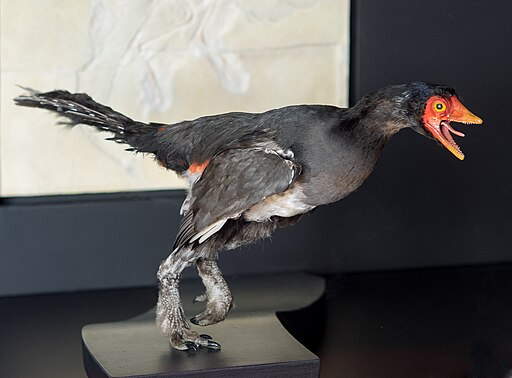
\includegraphics[width=0.8\textwidth]{figures/Archaeopteryx-Modell.jpg}
    \caption{A model of an Archaeopteryx, an early bird with teeth. Photo by Dr. Nachtigaller, CC BY-SA 4.0, \href{https://commons.wikimedia.org/wiki/File:Archaeopteryx-Modell.jpg}{via Wikimedia Commons.}}
    \label{fig:enter-label}
\end{figure}

Newer theories of categories offers a more nuanced way of understanding, but sometimes there's no getting away from a classical view. For example, laws often need to define the categories to which they apply. In most such cases, it's not possible to say the law applies sort of. In a dispute, there is ultimately a finding for or against the defendant, and this reflects the binary nature of the classical view. There are other reasons too.

The law often prioritizes certainty and predictability over fidelity to the natural world. Shifting completely to prototype-like models, where boundaries are fuzzier, could undermine the consistent application of justice that legal systems strive for. Legal systems heavily rely on precedent. Clearly defined categories allow for better comparison and consistency over time. Modern theories would lead to more subjective and potentially shifting definitions. Laws are, by their nature, written documents. They need some level of precision in language that classical category definitions provide more readily than prototype-like models.

Nevertheless, definitions are often omitted, leaving instead words such as \textit{fruit}, \textit{fish}, or \textit{refugee}, which have to be interpreted, a process that can end up being overly restrictive or overly vague.

The International Association of Athletics Federations (IAAF) had a rule disqualifying the use of ``technical aids'', but lacked a definition of what constituted such an aid. Oscar Pistorius, the double amputee runner known as the ``Blade Runner'' for his iconic carbon fiber prostheses applied to compete in the 2008 Olympics, but the IAAF blocked his bid, claiming that his prostheses qualified as technical aids. Pistorius challenged this decision.

The debate was complex. Scientific testing showed that the prostheses provided a unique rebound effect, differing from the energy return experienced by the other Olympic runners. But it wasn't clear-cut whether this constituted an overall advantage. Pistorius argued his disadvantage of lacking lower legs balanced any potential benefits of the blades. Ultimately the IAAF's interpretation was ruled to be too narrow, and he was allowed to compete.

An interpretation can be overly general, though. In 2005, Ontario enacted a law banning ``pit bulls''. The law was a response to public fear after a few high-profile attacks on Ontarians. Unfortunately, the law didn't define \textit{pit bull}. Nor did it provide a list of breeds or even a clearly stated set of physical characteristics. Enforcement became highly subjective.

Dogs were seized and transferred out of the province, euthanized, or turned over to a research facility, based on appearance alone, even if those dogs had no history of aggression. Dog owners feared for their pets, while critics argued the law targeted dogs, not dangerous behaviors. The law was later challenged in court, with experts arguing that identifying a dog as a pit bull was often impossible, even for trained professionals.

The term \textit{pit bull} lacks concrete definition. It's more of a catch-all, not a pedigreed breed. Ontario's overly vague law led to inconsistent application, unfair targeting of dogs, and failed to actually address the problem of dangerous dogs of any breed.

In Massachusetts, a legal battle over the categorization of a burrito unfolded between Panera Bread and Qdoba Mexican Grill. Panera Bread's lease agreement with the White City Shopping Center contained a clause prohibiting the mall from renting space to other sandwich restaurants. When Qdoba sought to open a location in the mall, Panera argued that Qdoba's burritos fell under the category of sandwiches, violating the lease agreement. The case, which reached the Worcester County Superior Court in 2006, centered on whether a burrito could be legally defined as a sandwich.

Chef and food writer Christopher Schlesinger testified, arguing against the sandwich classification for a burrito, noting the absurdity of such categorization to any credible chef or culinary historian. The court, guided by Merriam-Webster's definition, ruled in favor of Qdoba, stating that common sense and the dictionary definition of a sandwich -- as two slices of bread with fillings in between -- excluded burritos, tacos, and quesadillas from the category.

In one final example, the classification of Constantin Brancusi's ``Bird in Space'' as art or kitchen utensils by US customs in 1926 serves as another compelling narrative on categorization. Upon its arrival in New York for an exhibition, customs officials, adhering to a classical view of sculpture as imitative of natural objects, classified the abstract sculpture as a utilitarian object, subjecting it to import taxes. Brancusi challenged this classification in court, sparking a legal debate on the nature of art and sculpture.

\begin{wrapfigure}{r}{0.5\textwidth}
\centering
 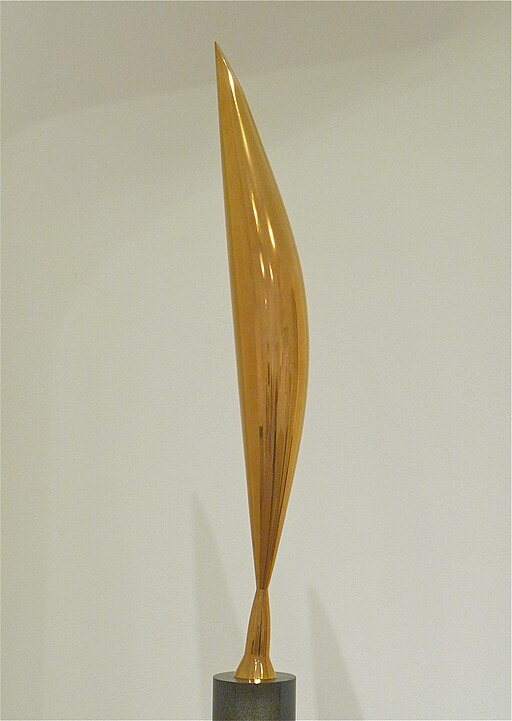
\includegraphics[width=0.48\textwidth]{figures/Bird_in_Space.jpg}
 \caption{Brancusi's Bird in Space. Image by Art Poskanzer, Public domain, via Wikimedia Commons.}
\end{wrapfigure}


The trial called upon expert testimonies, including those of artist Edward Steichen and art critic Frank Crowninshield, to argue for the sculpture's artistic merit beyond its non-representational form. The court eventually ruled in favor of Brancusi, acknowledging the evolving nature of art that transcends literal imitation of natural objects. This decision not only exempted Bird in Space from customs duties but also broadened the legal understanding of art, recognizing the legitimacy of abstract and avant-garde forms.

These cases underscore the classical view's limitations and strengths in categorization. While the classical approach provides a necessary foundation for legal and practical determinations, it also encounters challenges when faced with evolving societal and cultural norms. The resolution of these disputes reflects a broader legal and societal recognition of the need for definitions that accommodate changing perceptions and values, demonstrating compromises between the classical view and the nuanced reality of categorization.

When it comes to grammaticality, though, rarely is anyone called on to make a binding or fraught decision about whether or not something is grammatical, linguistics papers notwithstanding. As I've said before, most of the ungrammatical things that people say or write still clearly convey their intended meaning, and grammaticality is no guarantee of clarity.


\subsection{Prototypes theory}

A particularly good alternative to the classical view is prototype theory, especially when it comes to language. Think back to when you were a toddler, learning about birds. Someone might have pointed to a robin and said, ``That's a bird.'' Later, you saw other robins and called them ``bird'' too, no problem. But as time went on, things got a bit more complicated. You learned that ducks and chickens were also birds, and you had to learn that bats were not. Eventually, you found out about penguins and even ostriches. As your idea evolved, that original image of ``bird'' in your head didn't quite fit the bill anymore.

This is the kind of problem that Eleanor Rosch and her theory of prototypes aim to address. Instead of the traditional way of understanding categories -- with clear-cut definitions and strict membership rules -- Rosch proposed that our minds organize concepts in a much fuzzier way. She suggested that there are really good examples -- exemplars, prototypes -- that we put at the centre of our category concept and then we add less central members as we go.

In language, it's not just grammaticality that's fuzzy. Categories like adjective and noun are too. There are really good examples of adjectives like \textit{big}. They evoke a property of an object. They're gradable, \textit{big}, \textit{bigger}, \textit{biggest} and we can intensify them with adverbs like \textit{very}. They can be used before a noun \textit{a big deal} or after a verb \textit{the world is big}. \textit{Big} is a really good adjective. \textit{Worth} isn't.

If I say \textit{it's work your time}, then \textit{your time} is a grammatical object, but objects go with verbs and preposition, not adjectives. Also, you can't say *\textit{this is a worth initiative}; you have to say \textit{worthy} or \textit{worthwhile}. One thing isn't \textit{worther} and another. \textit{Worth} is the ostrich of adjectives or the bat of mammals.

\subsection{across time}

The progressive aspect (\textit{we'\uline{re going}}; \textit{I \uline{was trying}}; \textit{it'\uline{s happening}}) is newish in English. It's a construction that is generally formed with \textit{be} + the \textit{--ing} form of a verb and means that some situation is in progress or pertains at the time in question but is expected to end. Consider the difference between \textit{I live in Toronto} and \textit{I'\uline{m living} in Toronto}. Both sentences mean that I'm currently a resident of Toronto, but the second, with the progressive aspect, has the additional meaning that I see the city as my temporary abode, that, I didn't always live here, and sooner or later, I'll be moving on. It's the kind of thing an international student might say.

Of course nothing lasts forever, but the progressive aspect makes this explicit and draws our attention to it. It says, `this situation had a beginning and the end if foreseeable, and I thought you should know.' It's the aspect of the pragmatist who is aware of impermanence, the aspect of autumn.

But it's also about beginnings. Think about what it means to say \textit{I'\uline{m walking} to work every morning} compared to the simpler \textit{I walk to work every morning}. Both clearly convey my current means of commuting, but while the second is a mere statement of fact, the first suggests a tentativeness. Perhaps, I'm trying to exercise more -- I know the habit might not persist, but it's what I do now.

French and Italian don't have a progressive aspect the way English does, nor does German or a lot of other closely related languages. Of course, they can convey the progressive nature of a situation, beginnings and endings, just not with a progressive aspect with \textit{be} and a special form of the verb. More that that, though, it's just not really a conventional message. An Italian speaker would rarely go out of their way to convey the progressive meaning of \textit{I'm walking to work}. Even if the situations were the same, they would almost certainly stick to \textit{vado al lavoro a piedi} `I walk to work'.

\bigskip

I tell you this because, like all these other western European languages, English didn't used to have a present progressive, and the change was gradual. In other words, once the construction got started, there was a gradient of grammaticality across time and across the population at any given time. And those two types of gradience continue today as the progressive aspect expands the range of constructions with which it may interact.

As I said, our progressive aspect is newish. 400 years ago, Shakespeare had Hamlet say, ``O, I die, Horatio,'' not ``O, I'm dying, Horatio.'' Shakespeare's language is what experts call Modern English. It was preceded by Middle English and Old English, so that's why I say it's relatively new. Today, \textsuperscript{?}\textit{I die} verges/is verging on ungrammatical. Something has changed to this language we call Modern English.

Perhaps, what might save \textit{I die} today is its evocation, serious or facetious, of an earlier time, such a time signal being one possible meaning of a construction. The converse of this, though wouldn't work. Somebody in Shakespeare's time could not have evoked our present age by using the present progressive because no such construction existed. As such it could neither have conveyed a situation in progress with a delimited beginning and end nor a manner of speech typical of twenty-first century English. In other words, it's most likely that, in 1600, *\textit{I'm dying, Horatio} would have been ungrammatical.

How did the present progressive become grammatical? There wasn't a proclamation or any kind of phase transition. Instead, it progressed more or less the way science does: one death at a time. There was a slow accretion of younger users who learned the construction growing up and treated it as a natural part of the language. Some adults would have learned it and become comfortable with hearing it over time. Some may even have started using it.

The development was more or less that shown in (\ref{ex:a-hunting}), with modernized spelling.

\ea \label{ex:a-hunting}
 \ea[]{\textit{Yesterday I was on hunting.}\hfill Old English}
 \ex[]{\textit{Yesterday I was a-hunting.}\hfill Early Middle English}
 \ex[]{\textit{Yesterday I was hunting.}\hfill Later Middle English}
 \z
\z

The earliest use of \{\textit{be}\} \textit{trying} (including all forms of \textit{be}) in the Early English Books Online corpus is (\ref{ex:first-progressive}). I used \textit{trying} as an example because it's one of the most common verbs to appear in the progressive aspect today.

\ea[]{They \textit{had none other let or stop to kepe them out of Grece and asia, but only this, while they \uline{were trying} by the sworde;}\hfill1564}\label{ex:first-progressive}
\z

A second instance appears in 1592, four in the following decade, then one in the 1610s. As Figure \ref{fig:be-trying-eebo} shows, it's a slow launch, but remember that this corpus is limited by the number of English books available less than 200 years after the invention of the printing press. And what appears in books rarely represents the cutting edge of linguistic progress.

\begin{figure}[h!]
 \centering
 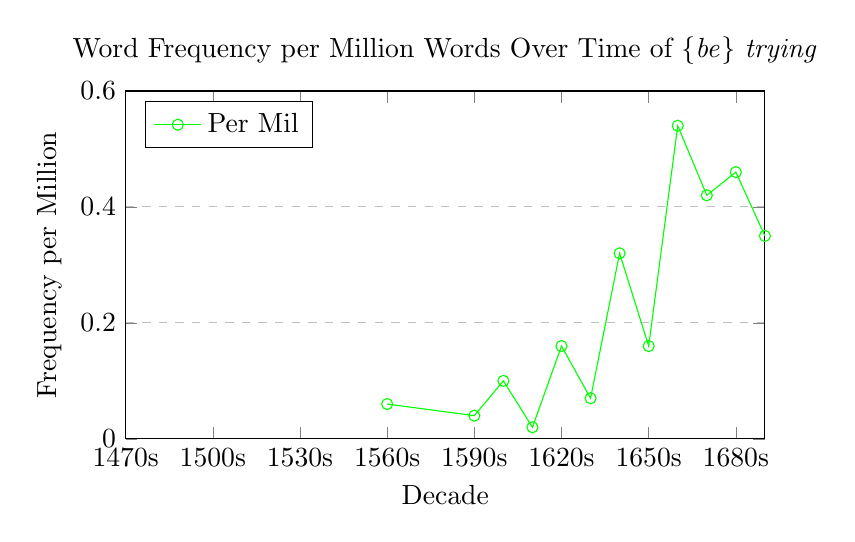
\begin{tikzpicture}
 \begin{axis}[
 title={Word Frequency per Million Words Over Time of \{\textit{be}\} \textit{trying}},
 xlabel={Decade},
 ylabel={Frequency per Million},
 xmin=1470, xmax=1690,
 ymin=0, ymax=0.6,
 xtick={1470,1500,1530,1560,1590,1620,1650,1680},
 xticklabels={1470s,1500s,1530s,1560s,1590s,1620s,1650s,1680s},
 legend pos=north west,
 ymajorgrids=true,
 grid style=dashed,
 width=0.8\textwidth, % Adjusts the width of the tikzpicture within the figure.
 height=6cm, % Adjust height as needed
 ]
 
 % Plot Per Mil
 \addplot[
 color=green,
 mark=o,
 ] coordinates {
 (1560,0.06)(1590,0.04)(1600,0.10)(1610,0.02)(1620,0.16)(1630,0.07)(1640,0.32)(1650,0.16)(1660,0.54)(1670,0.42)(1680,0.46)(1690,0.35)
 };
 \addlegendentry{Per Mil}
 \end{axis}
 \end{tikzpicture}
 \caption{Evolution of word frequency per million words from the 1560s to the 1690s.}\label{fig:be-trying-eebo}
\end{figure}

By 1820, \{\textit{be}\} \textit{trying} was up to about five instances per million words, and it has continued its spread, so that by the 2010s it was occurring close to 120 times per million words in the Corpus of Historical American English. But just because the progressive aspect had become somewhat common didn't mean that it was fully grammatical in all potential positions. What about combining with the perfect aspect, for example?

The perfect aspect is a construction that uses \{\textit{have}\} plus the past participle: \textit{he had tried}, \textit{I've got}, \textit{she's seen}, etc. The past participle of \textit{be} is \textit{been}, so, combining the perfect aspect with the progressive, we get \{\textit{have}\} \textit{been trying}. That ubiquitous and seems perfectly fine to us today, but it's actually not obvious that the two aspects can be combined. In fact, the opposite order *\textit{I'm having tried} is ungrammatical.

Another environment is the passive construction. Formally, the passive takes the \{\textit{be}\} of the progressive and the past participle of the perfect: \textit{I was born}, \textit{it's made}, \textit{people were told}. Combinging the perfect with the passive produces \textit{I was being born}, \textit{it's being made}, and \textit{people were being told}. These structure are also common.

But if we try to combine all three, we get the rather questionable \textsuperscript{?}\textit{I had been being born}, \textsuperscript{?}\textit{it has been being made}, and \textsuperscript{?}\textit{people had been being told.}

If that seems just a bit too complicated, what about just progressive \{\textit{be}\}? I'm OK with \textit{he's being a jerk}, but \textsuperscript{?}\textit{He seems to be being a jerk}? You might say \textit{I'm being provocative} but perhaps not \textsuperscript{?}\textit{I might be being a bit provocative.} And although \textit{they've been to Sweden} is fine, you'd never say \textit{they're being to Sweden}.

There are whole classes of verbs that express states and resist the progressive. It seems incongruous to say \textit{I'm knowing that}, and we can say explain this as a clash between the temporary meaning of the progressive construction and the enduring nature of knowledge. Even if we know the potential to forget something, it's difficult to imagine a situation in which one would want to convey the expectation that the knowledge will be temporary. But what about this one: somebody has just introduced themselves, and you know their name, but you also know you're not good at recalling the names later. Even in that situation, I can't get a grammatical feeling for *\textit{I'm knowing their names.}

Progressive \textit{know} does not seem to be on the rise in the Corpus of Historical English \citep{Granath2014}, though the data is sparse. Nevertheless, given it's partial and occasional grammaticality today, I would not be surprised to find that in another hundred years progressive aspect had become even more common and made inroads among the stative verbs.

Another point of gradience is between grammar and lexis.

\section{Everything is grammatical}

\citet{Sampson2014b} think that the whole idea of grammaticality is nonsense. According to them, there's no such thing. Or perhaps, to put it another way, they think the question of grammaticality simply reduces to the question of whether you can find an expression in a corpus: If it has been used, then it's grammatical. This is a deceptively simple but ultimately unsatisfying view. Nor does it match with most people's experience with grammaticality. It certainly doesn't explain my intuition about (\ref{ex:allowed-dessert}).

A key example illustrating their argument comes from the study of dialects. In the UK, the use of "I were" in a sentence like "I were there" might be deemed ungrammatical in Standard English, yet it is perfectly acceptable in certain regional dialects, such as those spoken in Yorkshire. This variation demonstrates language's adaptability to different social and regional contexts, challenging the notion of a single, uniform standard of grammaticality.